\chapter{Introduction}
\pagenumbering{arabic}
\section{Background} \hbadness=100000 
\sloppy
Steganography is the skillful technique of secret communication, accomplished through embedding a piece of information into a carrier. In steganography, a ``carrier'' refers to the cover or host file that conceals the hidden message or information. The word steganography is derived from the Greek words \textit{“stegos”} meaning \textit{“cover”} and \textit{“grafia”} meaning \textit{“writing”} defining it as \textit{“covered writing”} \cite{14}. Misusing steganography for malicious purposes can have serious consequences. A recent trend involves exploiting various steganographic techniques to embedd malware in the carrier. Some real life example would be: Hiding malicious code within banner ads, tricking users into installing malicious app, embedding malicious executables and so on. Steganography can utilize various file formats, primarily classified into four categories: text, images, audio, and video. Among these file formats, images are widely used as cover object.\\
Steganalysis is the process of detecting hidden information within digital media, uncovering hidden data that has been secretly embedded using steganographic techniques. The goal of steganalysis is to collect sufficient evidence about the presence of embedded message and to break the security of its carrier. Thus defeating the purpose of steganography. The importance of steganalytic techniques that can reliably detect the presence of hidden information in images is increasing. Steganalysis finds its use in computer forensics, cyber warfare, tracking the criminal activities over the internet and gathering evidence for investigations particularly in case of anti-social elements.\cite{20} \\ \\
\textbf{Image Steganography}\\
Image Steganography is a steganography method where the hidden information is embedded into a image as carrier file. Among the various available formats of images, JPEG format is widely used for steganography because of its lossy compression. The figure below shows the glimpse of how a JPEG image is compressed.\\
\begin{figure}[H]
    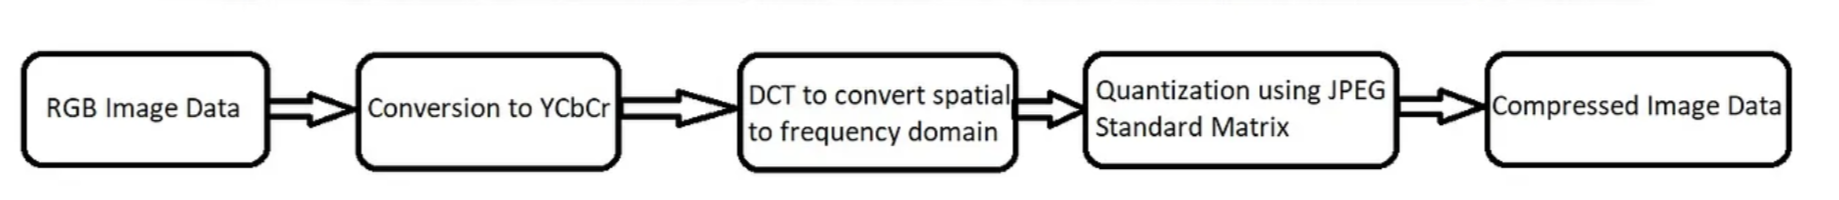
\includegraphics[width=1\textwidth]{./img/compression.png}\\
    \caption{ Steps used in implementation of Compression Algorithm}
\end{figure}
\begin{flushleft} 
\end{flushleft} 
First the RGB color space is converted into YCbCr colorspace. After the YCbCr coversion, the image is partitioned into 8$\times$8 non-overlapping blocks. After that each pixel is transfered from range of 0 to 255 to -128 to 127. Finally, Each of these blocks is then subjected to a 2-D Discrete Cosine Transform (DCT). The DCT transforms the spatial data in the block into frequency data. After the DCT, the coefficients are quantized, meaning they are divided by a factor determined by a quantization table. The quantization step is what actually removes information from the image, and it is this step that makes the JPEG compression process lossy.
\begin{equation} \label{eq:1.1} 
    C(u,v)=\alpha(u)\alpha(v)\sum_{x=0}^{N-1} \sum_{y=0}^{N-1} f(x,y) cos[\frac{\pi(2x+1)u}{2N}] cos[\frac{\pi(2y+1)v}{2N}]
\end{equation}
\hspace{1cm} for $u,v = 0,1,2,…,N-1$ and $f(x,y)$ is pixel position and $\alpha(u),\alpha(v)$ as 
\begin{equation}\label{eq:1.2}  
    \alpha(u)=\left\{\begin{matrix}
        \sqrt{\frac{1}{N}}& for & u=0 \\
        \sqrt{\frac{2}{N}}& for & u\neq 0 \\
       \end{matrix}\right.
\end{equation}
\begin{equation}\label{eq:1.3}   
    \alpha(v)=\left\{\begin{matrix}
        \sqrt{\frac{1}{N}}& for & v=0 \\
        \sqrt{\frac{2}{N}}& for & v\neq 0 \\
       \end{matrix}\right.
\end{equation}
Equation (\ref{eq:1.1}), (\ref{eq:1.2}), (\ref{eq:1.3}) are the formulas to calculate DCT coefficients, $\alpha(u)$ and $\alpha(v)$ respectively.\cite{4}\\ \\
Some popular techniques of image steganography are listed below: 
\begin{enumerate}  
    \item \textbf{DCT-LSB Method:}\\ The DCT-LSB method conceals data in an image by dividing it into 8x8 blocks, transforming each block using Discrete Cosine Transform (DCT), and then replacing the least significant bit of DCT coefficients with hidden data.\cite{16}
  
    \item \textbf{F5 and nsF5 Algorithms:}\\ The F5 steganography algorithm operates by manipulating Discrete Cosine Transform (DCT) coefficients. F5 adjusts coefficients by adding 1 to those with a positive value and subtracting 1 from those with a negative value, leaving zero-valued coefficients unchanged. However, a drawback known as the ``shrinkage'' problem arises when coefficients with values of 1 or -1 become zero during embedding, reducing the algorithm's capacity.\cite{17}\\To overcome the shrinkage problem, the nsF5 algorithm, an advanced version of F5, employs Wet Paper Codes (WPC). This technique designates certain coefficients as ``non-modifiable'', preventing alterations after data embedding. This innovation addresses the shrinkage issue without sacrificing capacity. Even if new zeros are generated from coefficients with values of 1 or -1, the nsF5 algorithm records them, enhancing image quality and capacity compared to the common F5 method.\cite{12}
  
    \item \textbf{UERD (Universal Embedding Reduced Distortion):}\\UERD (Universal Embedding Reduced Distortion) is a method that hides information in pictures so that it's hard to notice.By strategically analyzing Discrete Cosine Transform (DCT) coefficients, UERD chooses those areas in the picture where changes won't be obvious. UERD uses syndrome trellis coding (STC) to hide the message bits in the desired values. This further increases the security of the embedded data by making it harder to detect.\cite{13}  
    \item \textbf{J-UNIWARD Algorithm:}\\The J-UNIWARD algorithm operates in both the spatial domain and the frequency domain. In the spatial domain, it uses the Least Significant Bit (LSB) steganography technique to hide data in the least significant bits of the pixel values. In the frequency domain, it uses the Discrete Cosine Transform (DCT) to transform the image into the frequency domain, where it hides data in the DCT coefficients.\cite{22}
  
    \item \sloppy \textbf{HUGO Algorithm:}\\ HUGO, which stands for Highly Undetectable steGO, is a steganography algorithm designed to hide information within images. It achieves this by analyzing complex patterns and structures in an image, determining optimal locations to hide data.\cite{18}\cite{19}
  \end{enumerate}
\section{Motivation}
As motivated by the pressing need to combat cyber threats posed by the continuous evolution of steganography, which presents a serious threat to digital privacy and security, steganalysis tools have been used to detect embedded malicious content in an image. Given the extensive usage of images in digital communication, the use of advanced steganographic techniques in image files expose users to risk by concealing malicious data in easily accessible images. The increasing sophistication of steganographic techniques presents a challenge to traditional steganalysis approaches. This constitutes a significant risk of malicious data infiltration. To overcome this problem, new approaches must be investigated to accurately detect malicious data. By investigating steganalysis using ensemble classifiers, we aim to further strengthen the defenses against sophisticated steganographic attacks while maintaining computational efficiency.\\

\section{Problem Statement} 
The continuous evolution of steganographic techniques poses a critical challenge to digital privacy. Since two-thirds of the internet comprises of images and play a major role in digital communication, there is a considerable risk of exploitation through steganography. With the increasing sophistication of methods used to embed information secretly, traditional steganalysis approaches struggle to accurately detect and mitigate the risks associated with concealed malicious content. There is a pressing need for proper steganalysis techniques that can effectively identify and minimize the risks posed by hidden data embedding. Additionally, as steganography becomes more prevalent in digital communication, there is a growing need to develop robust steganalysis tools capable of detecting hidden information.\\
A notable example highlighting the need is the nefarious activities of the Witchetty espionage group, also known as LookingFrog. This group has demonstrated the malicious potential of steganography by compromising the security of Middle Eastern governments and the stock market in African countries by exploiting vulnerabilities using the Windows logo as a point of entry.\\
To address these problems, there’s a critical need for advanced and flexible steganalysis methodology. These tools must be competent in detecting hidden information embedded in digital images. This project aims to develop steganalysis model using ensemble classifiers to specifically detect hidden data within images. Through the integration of ensemble classifiers, the system will enhance detection capabilities by aggregating decisions from multiple base classifiers, thereby improving accuracy and robustness in identifying alterations indicating steganographic manipulation. 
\\
\clearpage

\section{Objectives}
The main objectives of this project is to:
\begin{itemize}
\item  To detect steganographically modified JPEG images using Ensemble \mbox{Classifier}, irrespective of the following algorithm used for steganography (nsf5,J-uniward,UERD). 
\end{itemize}
\section{Scope and application}
The major applications of this project are:
\begin{itemize}
    \item Organizations can employ steganalysis to detect malicious activities such as malware distribution or covert communication channels used by cybercriminals.
\end{itemize}

